\chapter{Exponential Decay}

In a previous chapter, we saw that an investment of $P$ getting
compound interest with an annual interest rate of $r$, grows
exponentially. At the end of year $t$, your balance would be

$$P\left(1 + r\right)^t$$

Because $r$ is positive, this number grows as time passes. You get a
nice exponential growth curve that looks something like this:
\begin{figure}[htbp]
    \centering
    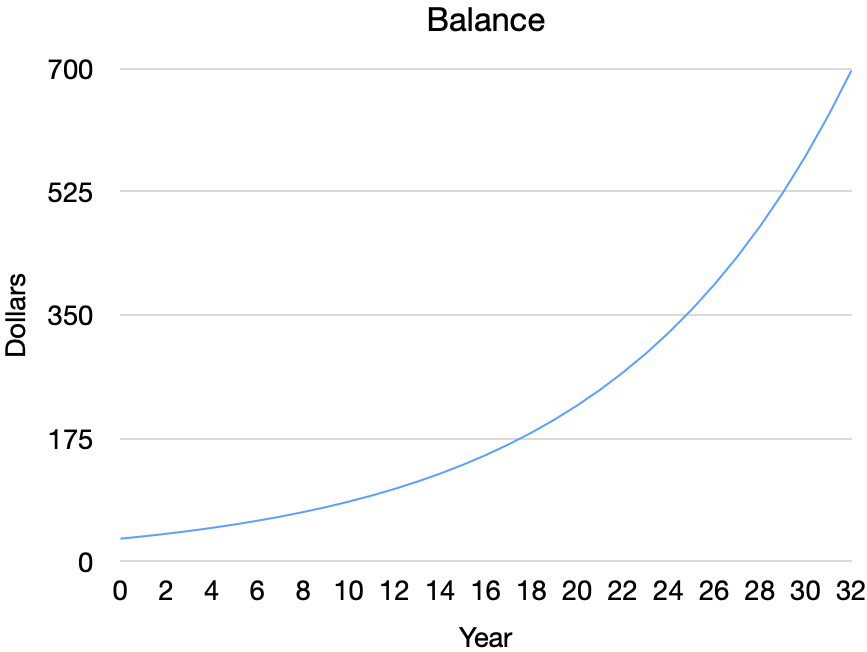
\includegraphics[width=0.7\textwidth]{exponential_growth.png}
    \caption{A diagram showing (exponential) compound interest.}
    \label{fig:exponential_growth}
\end{figure}

This is \$30 invested with a 10\% annual interest rate. So, the formula
for the balance after $t$ years would be

$$(30)(1.1)^t$$

What if $r$ were negative? This would be \textit{exponential decay}.

\section{Radioactive Decay}

Until around 1970, there were companies making watches whose faces and
hands were coated with radioactive paint. The paint usually contained
radium. When a radium atom decays, it gives off some energy, loses two
protons and two neutrons, and becomes becomes a different element
(radon). Some of the energy given off is visible light. Thus, these
watches glow in the dark.\index{radioactive decay}

How many of the radium atoms in the paint decay each century? About 4.24\%.

Notice the quantity of atoms lost is proportional to the number of
atoms you have. This is exponential decay. If we assume that we start
with a million radium atoms, the number of atoms decreases over time like this:
\begin{figure}[htbp]
    \centering
    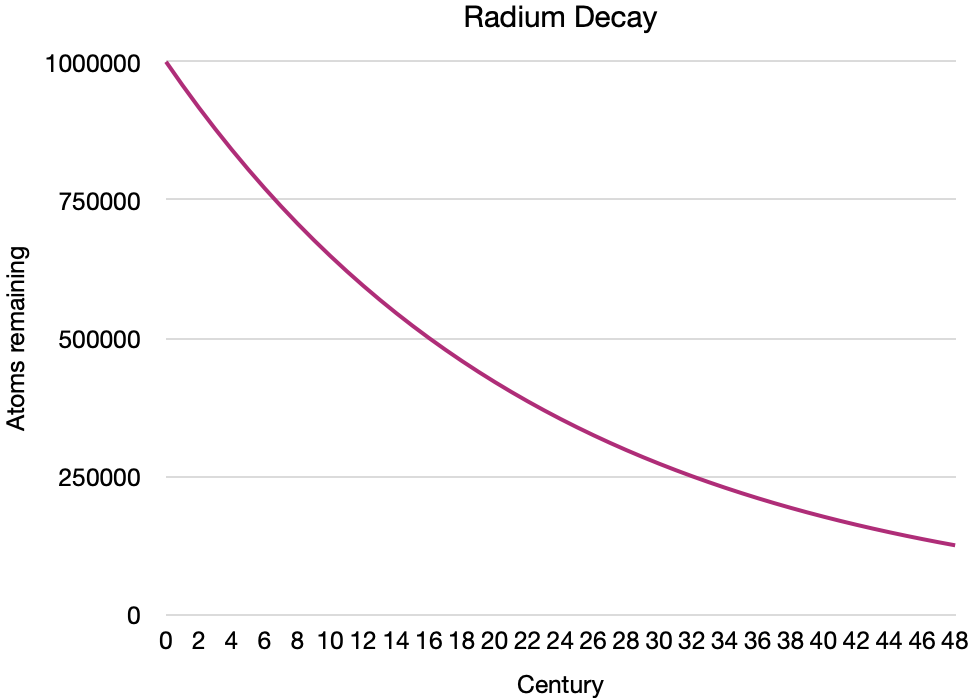
\includegraphics[width=0.7\textwidth]{radium_decay.png}
    \caption{A diagram showing the decay and half life of radium.}
    \label{fig:radium_decay}
\end{figure}
 
\begin{itemize}
\item We start with 1,000,000 atoms.
\item At 16 centuries, we have only 500,000 (half as many) left.
\item 16 centuries after that, we have only 250,000 (half again) left.
\item 16 centuries after that, we have only 125,000 (half again) left.
\end{itemize}

A nuclear chemist would say that radium has a \textit{half-life} of
1,600 years; its lifespan decreases by half its original amount every 1,600 years. Note that this means that if you bought a watch with
glowing hands in 1960, it will be glowing half as brightly in the year
3560.\index{half-life}

How do we calculate the amount of radium left at the end of century
$t$? If you start with $P$ atoms, at the end of the $t$-th century, you
will have

$$P\left(1 - 0.0424\right)^t$$

This is exponential decay.\index{exponential decay}
% 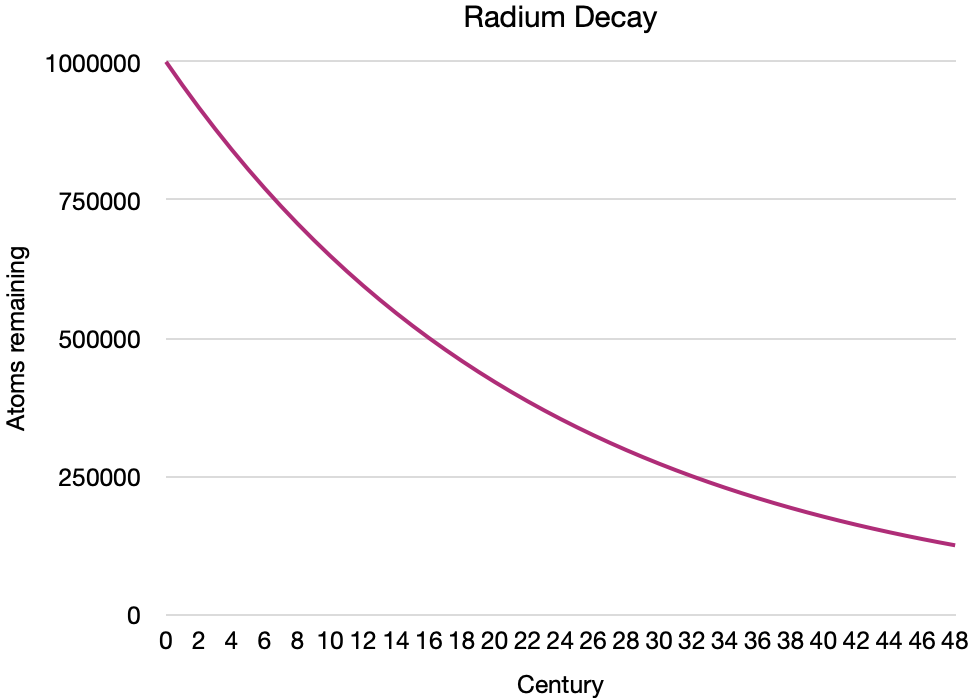
\includegraphics[width=0.7\textwidth]{radium_decay.png} INLCUDED Twice

\section{Model Exponential Decay}

Let's say you get hired to run a company with 480,000
employees. Each year, $1/8$ of your employees leave the company for
one reason or another (retirement, quitting, etc.). For some reason, you never
hire any new employees.

Make a spreadsheet that indicates how many of the original 480,000
employees will still be around at the end of each year for the next 12. Next, make a
bar graph from that data.

%FIXME finish this chapter?